\documentclass[border=10pt]{standalone}
\usepackage{amsmath}
\usepackage{tikz}
\usetikzlibrary{arrows.meta, positioning, fit, backgrounds, calc}

\definecolor{inputcol}{HTML}{4FC3F7}
\definecolor{modelcol}{HTML}{AB47BC}
\definecolor{toolcol}{HTML}{FFA726}
\definecolor{outputcol}{HTML}{66BB6A}

\begin{document}
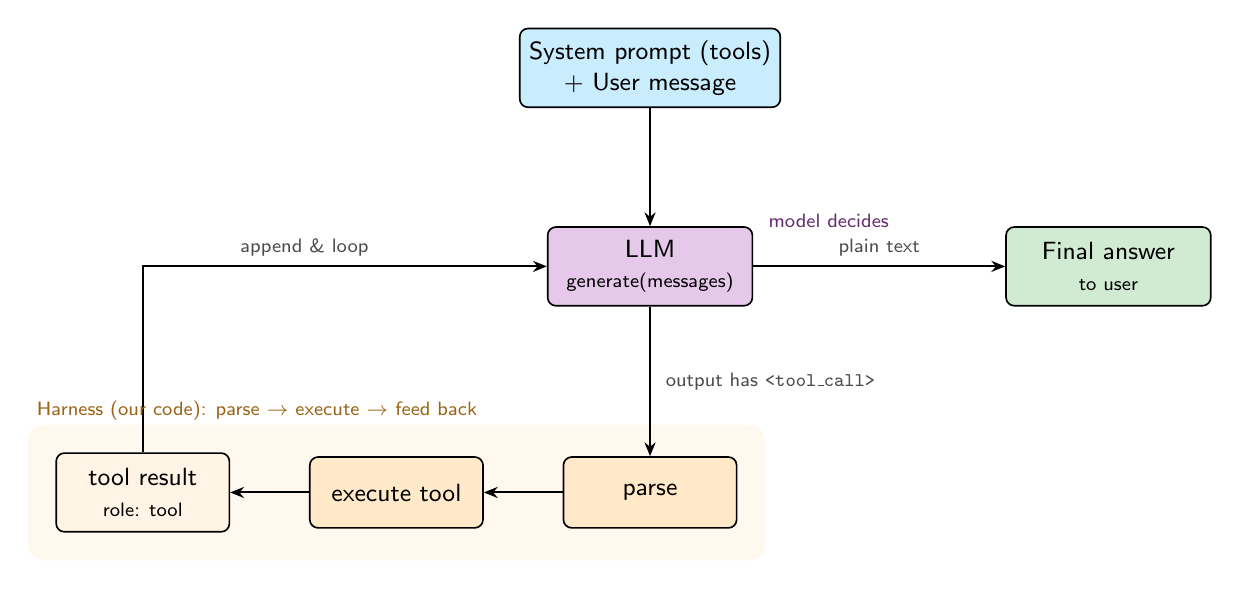
\begin{tikzpicture}[
  box/.style={draw, rounded corners=3pt, minimum width=2.6cm, minimum height=1.0cm,
    font=\sffamily\small, align=center, line width=0.6pt},
  op/.style={draw, rounded corners=3pt, minimum width=2.2cm, minimum height=0.9cm,
    font=\sffamily\small, align=center, line width=0.6pt, fill=toolcol!25},
  conn/.style={-{Stealth[length=5pt, width=4pt]}, line width=0.7pt},
  annot/.style={font=\sffamily\scriptsize, text=gray!60!black},
]

% Model in the center
\node[box, fill=modelcol!30] (model) {LLM\\ \scriptsize generate(messages)};

% Input above the model
\node[box, fill=inputcol!30, above=1.5cm of model] (inbox) {System prompt (tools)\\ + User message};

% Final answer to the right
\node[box, fill=outputcol!30, right=3.2cm of model] (final) {Final answer\\ \scriptsize to user};

% Harness chain (our code) below the model
\node[op, below=1.9cm of model] (parse) {parse};
\node[op, left=1.0cm of parse] (exec) {execute tool};
\node[box, fill=toolcol!12, left=1.0cm of exec, minimum width=2.2cm] (toolres) {tool result\\ \scriptsize role: tool};

% input -> model
\draw[conn] (inbox) -- (model);
% model -> final (no tool call)
\draw[conn] (model) -- node[annot, above] {plain text} (final);
% model -> parse (has tool call)
\draw[conn] (model.south) -- node[annot, right=2pt] {output has \texttt{<tool\_call>}} (parse.north);
% parse -> execute -> tool result
\draw[conn] (parse) -- (exec);
\draw[conn] (exec) -- (toolres);
% feedback: tool result -> back into model (append to messages, loop)
\draw[conn] (toolres.north) |- node[annot, above, pos=0.7] {append \& loop} (model.west);

% Group harness box
\begin{scope}[on background layer]
  \node[fit=(parse)(exec)(toolres), fill=toolcol!8, rounded corners=6pt,
        inner sep=10pt] (harness) {};
\end{scope}
\node[annot, text=toolcol!60!black, anchor=north west] at (harness.north west) [yshift=12pt]
  {Harness (our code): parse $\to$ execute $\to$ feed back};

\node[annot, text=modelcol!60!black, right=2pt of model.north east, yshift=2pt] {model decides};

\end{tikzpicture}
\end{document}
